\documentclass[portrait,a0]{a0poster}
\usepackage{color,multicol}
\usepackage[english]{babel}
\usepackage[utf8]{inputenc}
\usepackage[T1]{fontenc}
\usepackage{siunitx}
\usepackage{graphicx}
\usepackage{booktabs}
%\usepackage[round]{natbib}
\usepackage[font=small]{caption}
\usepackage{lmodern}
\usepackage[overload]{textcase}
\usepackage{setspace}
\usepackage{float}
\usepackage{titlesec}
\usepackage{lipsum} % Lorem ipsum generator
\usepackage{caption}
\usepackage{tikz}


\columnsep = 50pt % change this for separation of the columns

\definecolor{facultyColor}{cmyk}{0,.37,.88,.02} % faculty of science
\definecolor{gray}{cmyk}{.13,.05,0,.25}

\titleformat{\section}[hang]
{\LARGE\usefont{T1}{phv}{bx}{n}\color{facultyColor}} % format
{} % label
{0pt} % sep
{\MakeUppercase} % before-code

\begin{document}

\large

%\vspace*{\fill} %some more marginal up

%\begin{minipage}[t]{0.98\linewidth} % The first minipage for the logo & title
%\vspace{0pt} % A trick to align the parallel minipages on top

%\vspace{0.008\linewidth} % Increase the top margin
%\begin{multicols}{2} 
\begin{minipage}[t]{.4\linewidth} % logo
\vspace{0pt} % Alingns the parallel minipages on top

\includegraphics[height=0.35\linewidth]{HYlogo_fac_text-en}
\hspace{50pt}
%\includegraphics[width=0.35\linewidth]{division}
\end{minipage} % no empty line before the next begin

\vspace{-10cm}

\begin{minipage}[t]{.98\linewidth} % logo
\vspace{0pt} % Alingns the parallel minipages on top
\begin{flushright}
\begin{spacing}{5}
%{\usefont{T1}{phv}{bx}{n}\textcolor{facultycolor}{\MakeUppercase{Faculty of Science}} \MakeUppercase{}} 
%{\Huge\usefont{T1}{phv}{bx}{n}\textcolor{black}{\MakeUppercase{Helsingin Yliopisto}} \MakeUppercase{}}\\
%{\Huge\usefont{T1}{phv}{bx}{n}\textcolor{black}{\MakeUppercase{Helsingfors Universitet}} \MakeUppercase{}}\\
{\huge\usefont{T1}{phv}{bx}{n}\textcolor{black}{\MakeUppercase{University of Helsinki}} \MakeUppercase{}}\\
%{\Huge\usefont{T1}{phv}{bx}{n}\textcolor{facultyColor}{\MakeUppercase{Matemaattis-Luonnontieteellinen tiedekunta}} \MakeUppercase{}}\\
%{\Huge\usefont{T1}{phv}{bx}{n}\textcolor{facultyColor}{\MakeUppercase{Matematisk-Naturvetenskapliga fakulteten}} \MakeUppercase{}}\\
{\huge\usefont{T1}{phv}{bx}{n}\textcolor{facultyColor}{\MakeUppercase{Faculty of Science}} \MakeUppercase{}}\\
{\Large\usefont{T1}{phv}{bx}{n}\textcolor{facultyColor}{{Department of Computer Science}}{}}\\
\end{spacing}
\end{flushright}
\hspace{50pt}

\end{minipage} % no empty line before the next begin

%\end{minipage}

%\end{multicols}


\begin{multicols}{2} 
\begin{minipage}[t]{1.5\linewidth}
\vspace{10pt}
\begin{flushleft}
\begin{spacing}{5}
%\begin{center}
% Highlight two first words of the title with the faculty color
%%%%%%%%%%%%{\huge\usefont{T1}{phv}{bx}{n}\textcolor{blue}{\MakeUppercase{Defeating Downgrade Attack on Identity Privacy in 5G}} \MakeUppercase{}} \\

%\end{center}
\end{spacing}
\end{flushleft}
\end{minipage}

\begin{minipage}[t]{.95\linewidth} % title
\vspace{-110pt} % Alingns the parallel minipages on top
\begin{flushright}
\textsf{\bfseries
Mohsin Khan%$^\textbf{1}$ 
\\
%Kimmo Järvinen$^\textbf{1}$\\
%Philip Ginzboorg$^\textbf{2}$\\
Valtteri Niemi%$^\textbf{1}$\\
} % Text size for a1 posters
%\textcolor{gray}{\textsf{\bfseries{$^\textbf{1}$Department of Computer Science, University of Helsinki}}}\\
%\textcolor{gray}{\textsf{\bfseries{$^\textbf{2}$Huawei Technologies}}}
\end{flushright}
\end{minipage}
\end{multicols}


\vspace{30pt}

\begin{center}
 {\Huge\usefont{T1}{phv}{bx}{n}\textcolor{black}{\MakeUppercase{Identity Privacy in 5G, Defeating Downgrade Attack}} \MakeUppercase{}}
\end{center}

%\end{minipage}
\vspace{20pt}
%\vfill % some more marginal between header and text
\noindent\makebox[\linewidth]{\rule{\paperwidth}{5pt}}

\begin{multicols}{2} % change this for different number of columns

\section{IMSI}

\begin{Large}
 
\end{Large}


\begin{itemize} \Large
 \item Stands for International Mobile Subscriber Identity.
 \item Globally Unique
 \item Also called SUPI in 5G
\end{itemize}

\vspace{30pt}

\begin{center}
    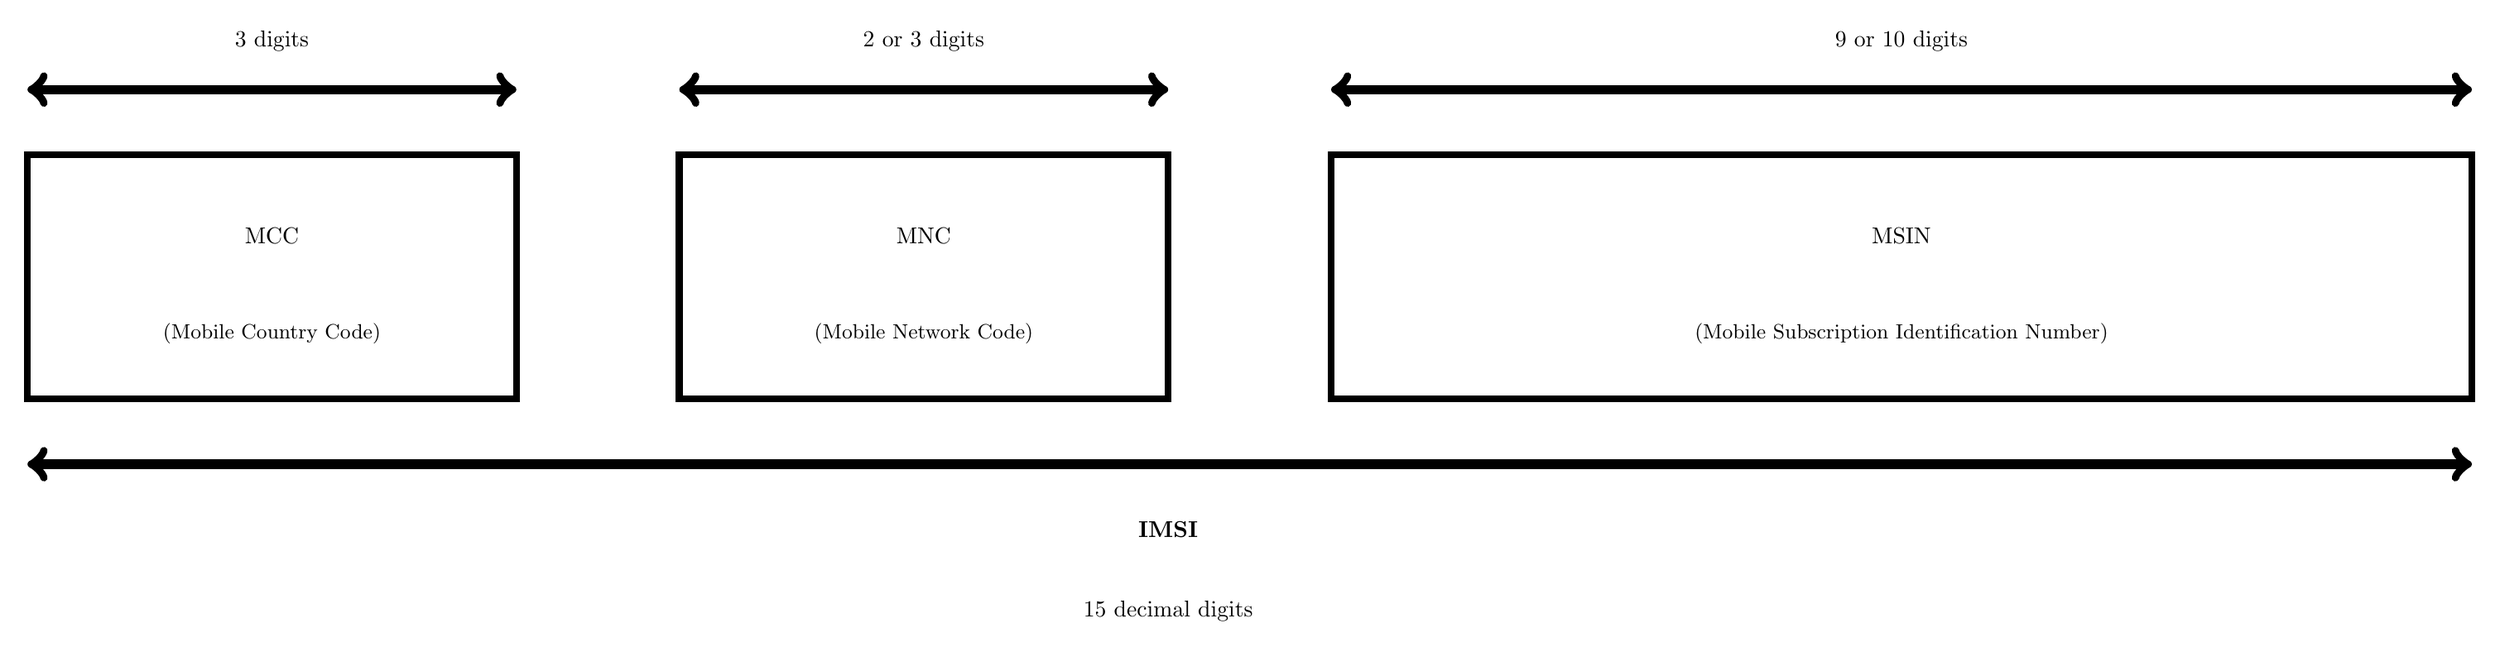
\begin{tikzpicture}[scale=5]



\filldraw[draw=black,fill=white,line width = 3pt] (0,0) rectangle (1.5,.75);
\draw [black, line width = 4pt, <->] (0,.95) -- (1.5,.95);
\draw node at (.75,1.1) {3 digits};
\draw node at (.75,.5) {MCC};
\draw node at (.75,.2) {\small (Mobile Country Code)};

\filldraw[draw=black,fill=white,line width = 3pt] (2,0) rectangle (3.5,.75);
\draw [black, line width = 4pt, <->] (2,0.95) -- (3.5,0.95);
\draw node at (2.75,1.1) {2 or 3 digits};
\draw node at (2.75,.5) {MNC};
\draw node at (2.75,.2) {\small (Mobile Network Code)};

\filldraw[draw=black,fill=white,line width = 3pt] (4,0) rectangle (7.5,.75);
\draw [black, line width = 4pt, <->] (4,0.95) -- (7.5,0.95);
\draw node at (5.75,1.1) {9 or 10 digits};
\draw node at (5.75,.5) {MSIN};
\draw node at (5.75,.2) {\small (Mobile Subscription Identification Number)};

\draw node at (3.5,-.4) {\textbf{IMSI}};
\draw node at (3.5,-.65) {15 decimal digits};


\draw [black, line width = 4pt, <->] (0,-0.2) -- (7.5,-0.2);

\end{tikzpicture}


\end{center}




\section{Passive IMSI Catchers}

\begin{Large}
A passive IMSI catcher is always listening and waiting for an IMSI to be sent in plaintext.
\end{Large}

\begin{center}
    \begin{tikzpicture}[scale=3]


\node[inner sep=0pt] (wsn) at (12,12)
    {
\includegraphics[height = 3cm]{home_network.jpg}};
\draw node at (12,11.2) {\textbf{HN}};

\draw [black, line width = 4pt] (12,11) -- (12,8);

\node[inner sep=0pt] (wsn) at (6,12)
    {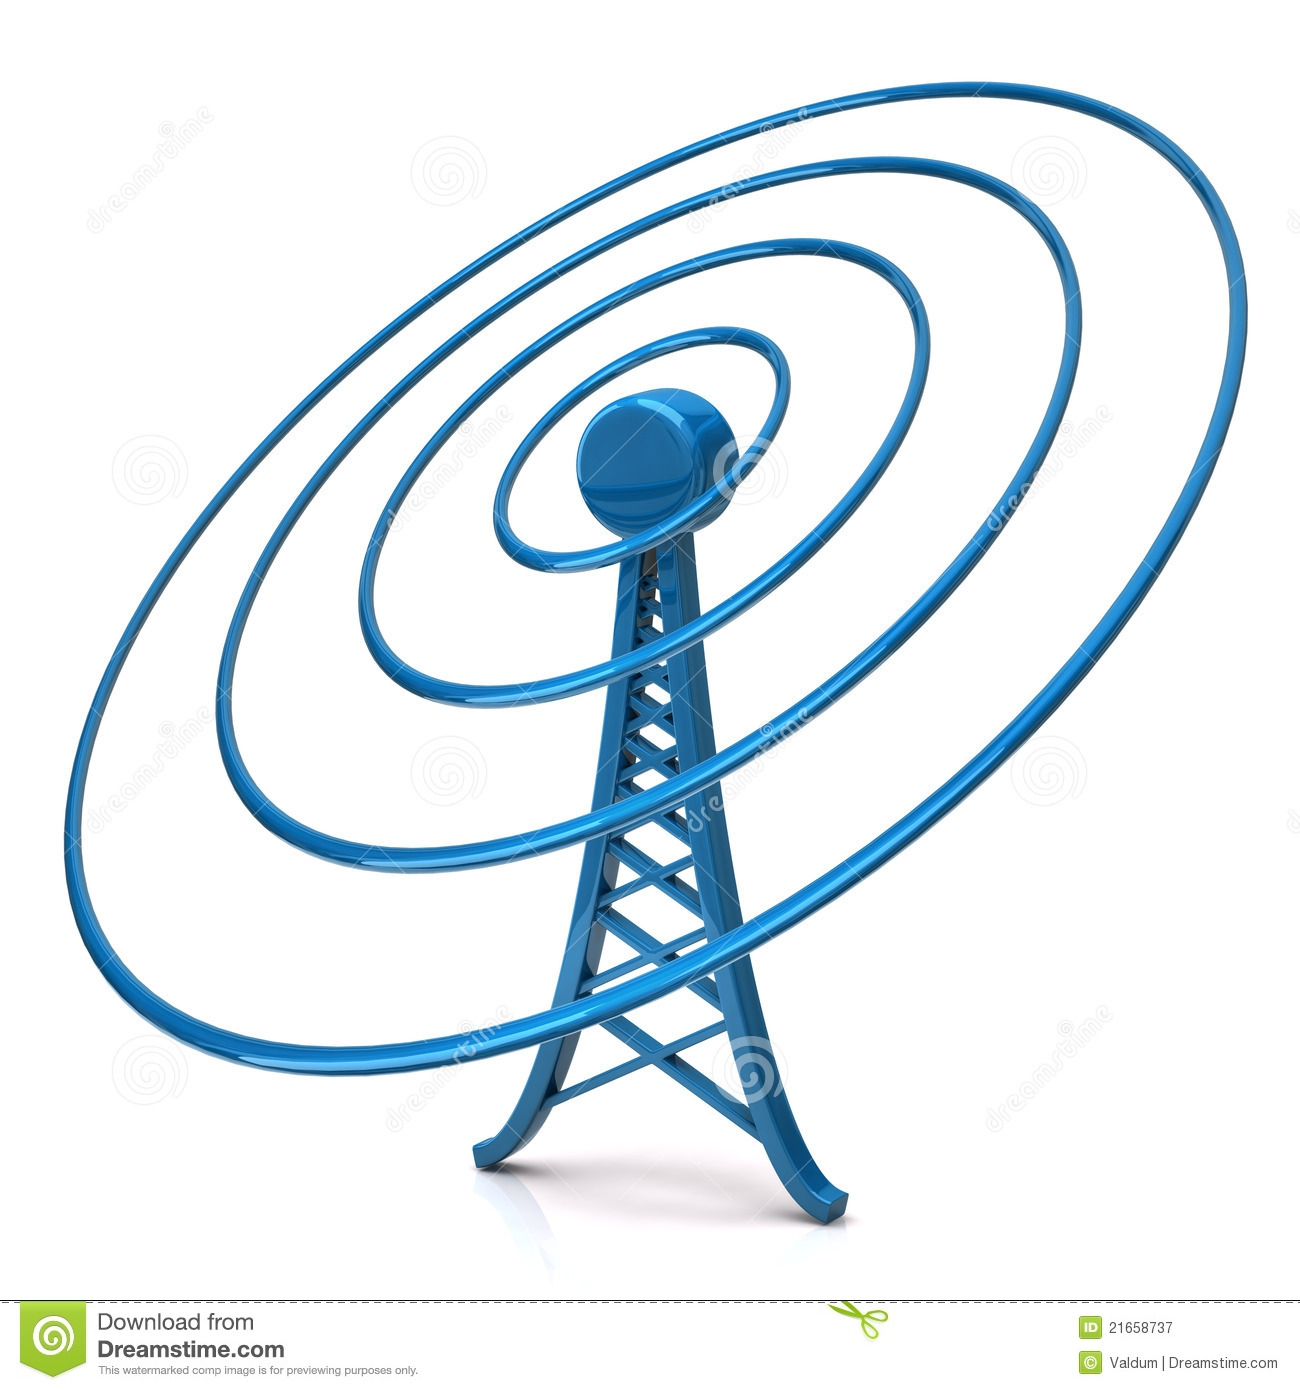
\includegraphics[height = 3cm]{tower.jpg}};
\filldraw[draw=white,fill=white] (4.5,11.25) rectangle (6.5,11.6);

\draw node at (6,11.2) {\textbf{SN}};

\draw [black, line width = 4pt] (6,11) -- (6,8);



\node[inner sep=0pt] (wsn) at (0,11.9)
    {
\includegraphics[height = 3cm]{smartphone.png}};
\draw node at (0,11.2) {\textbf{UE}};


\draw [black, line width = 4pt] (0,11) -- (0,8);


\draw [black, line width = 4pt, ->] (6.0,10) -- (0,10);
\draw node at (3.0,10.5) {\small Want to use the service?};
\draw node at (3.0,10.2) {\small Reveal your \textbf{IMSI} so that you can be billed.};


\draw [black, line width = 4pt, <-] (6,9) -- (0,9);
\draw node at (3,9.2) {\small \textbf{IMSI}};

\node[inner sep=0pt] (wsn) at (3,12)
    {
\includegraphics[height = 3cm]{listening_tower.png}};
\draw node at (3,11.2) {\small \textbf{\textcolor{red}{Passive IMSI Catcher}}};
\draw node at (3,10.9) {\small \textbf{\textcolor{red}{Evesdropping only}}};

\filldraw[-, dotted, fill opacity=0.1, cyan,line width = 3pt] (3,12.3) arc (90:450:2.5);


\end{tikzpicture}


\end{center}

\begin{Large} Protected in GSM, 3G and LTE. It will be protected in 5G too. \end{Large}
                                                                                                                                                                     


\section{Active IMSI Catchers}
\begin{Large}
An active IMSI catcher impersonates a legitimate SN.
\end{Large}

\begin{center}
    \begin{tikzpicture}[scale=2.75]


\node[inner sep=0pt] (wsn) at (12,12)
    {
\includegraphics[height = 3cm]{home_network.jpg}};
\draw node at (12,11.2) {\textbf{HN}};

\draw [black, line width = 4pt] (12,11) -- (12,8.3);

\node[inner sep=0pt] (wsn) at (6,12)
    {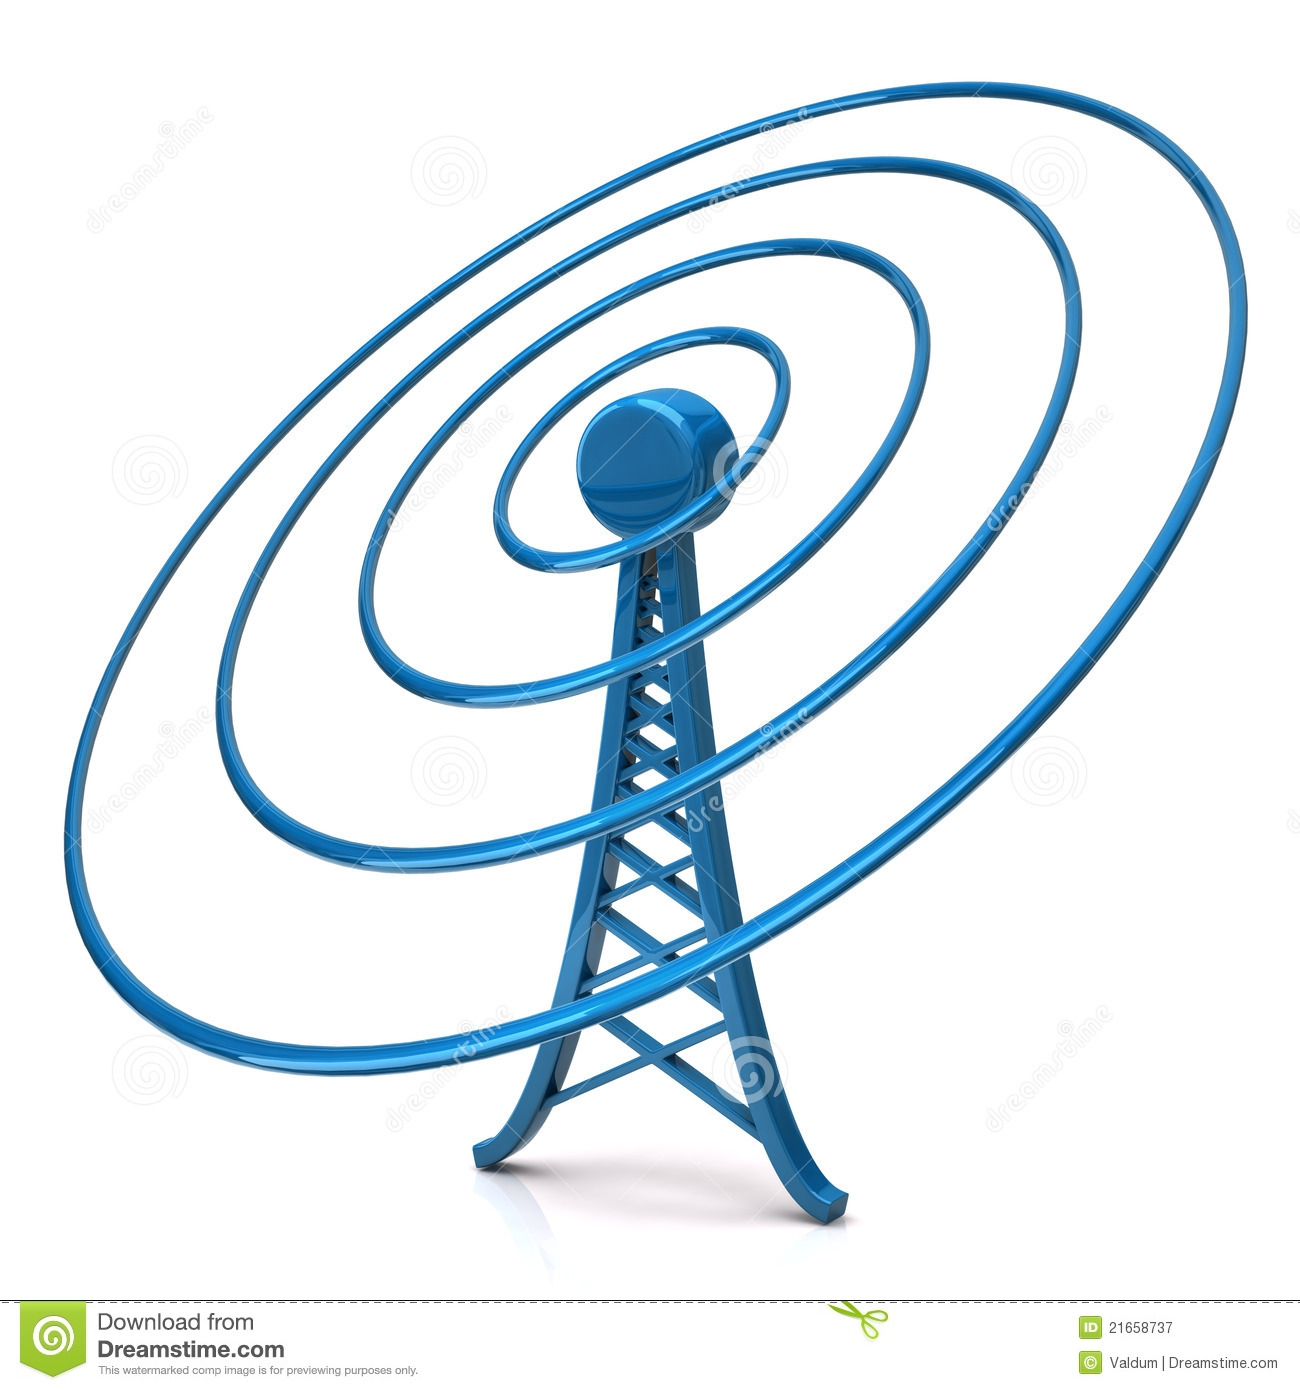
\includegraphics[height = 3cm]{tower.jpg}};
\filldraw[draw=white,fill=white] (4.5,11.25) rectangle (6.5,11.6);

\draw node at (6,11.2) {\textbf{SN}};

\draw [black, line width = 4pt] (6,11) -- (6,8.3);

\node[inner sep=0pt] (wsn) at (0,11.9)
    {
\includegraphics[height = 3cm]{smartphone.png}};
\draw node at (0,11.2) {\textbf{UE}};

\draw [black, line width = 4pt] (0,11) -- (0,8.3);


%\draw [black, line width = 3pt, <->] (6.0,10) -- (0,10);
%\draw node at (3.0,10.2) {\small Established connection};


\draw [black, line width = 4pt, ->] (4,9.7) -- (0,9.7);
\draw node at (2,10.5) { Stronger Signal};
\draw node at (2,10.1) { Reveal \textbf{IMSI}};

%\draw [black, line width = 3pt, <->] (6.0,8) -- (0,8);
%\draw node at (1.5,8) {\Huge \textcolor{red}{$\times$}};

\draw [black, line width = 4pt, <-] (4,8.7) -- (0,8.7);
\draw node at (2,9.1) {\textbf{IMSI}};


\node[inner sep=0pt] (wsn) at (4,12)
    {
\includegraphics[height = 3cm]{listening_tower.png}};
\draw [red, line width = 2pt,dotted,] (4,10.7) -- (4,8.3);
\draw node at (4,11.2) {\small \textbf{\textcolor{red}{Fake SN}}};
\draw node at (4,10.9) {\small \textbf{\textcolor{red}{Active IMSI Catcher}}};




\end{tikzpicture}


\end{center}

\begin{Large} There is no protection against against active IMSI catchers in GSM, 3G and LTE. There will be a protection in 5G. \end{Large}

\section{Defeating IMSI Catchers in 5G (Standardized)}
\begin{Large} 3GPP has decided to solve the problem using public-key encryption as follows. \end{Large}
\begin{center}
    \begin{tikzpicture}[scale=2.75]


\node[inner sep=0pt] (wsn) at (12,12)
    {
\includegraphics[height = 3cm]{home_network.jpg}};
\draw node at (12,11.2) {\textbf{HN(5G)}};

\draw node at (10.6,13.5) { HN's public key: $\mathit{pk}$};
\draw node at (10.7,13) {HN's private Key: $\mathit{sk}$};

\draw [black, line width = 4pt] (12,11) -- (12,7.75);

\node[inner sep=0pt] (wsn) at (6,12)
    {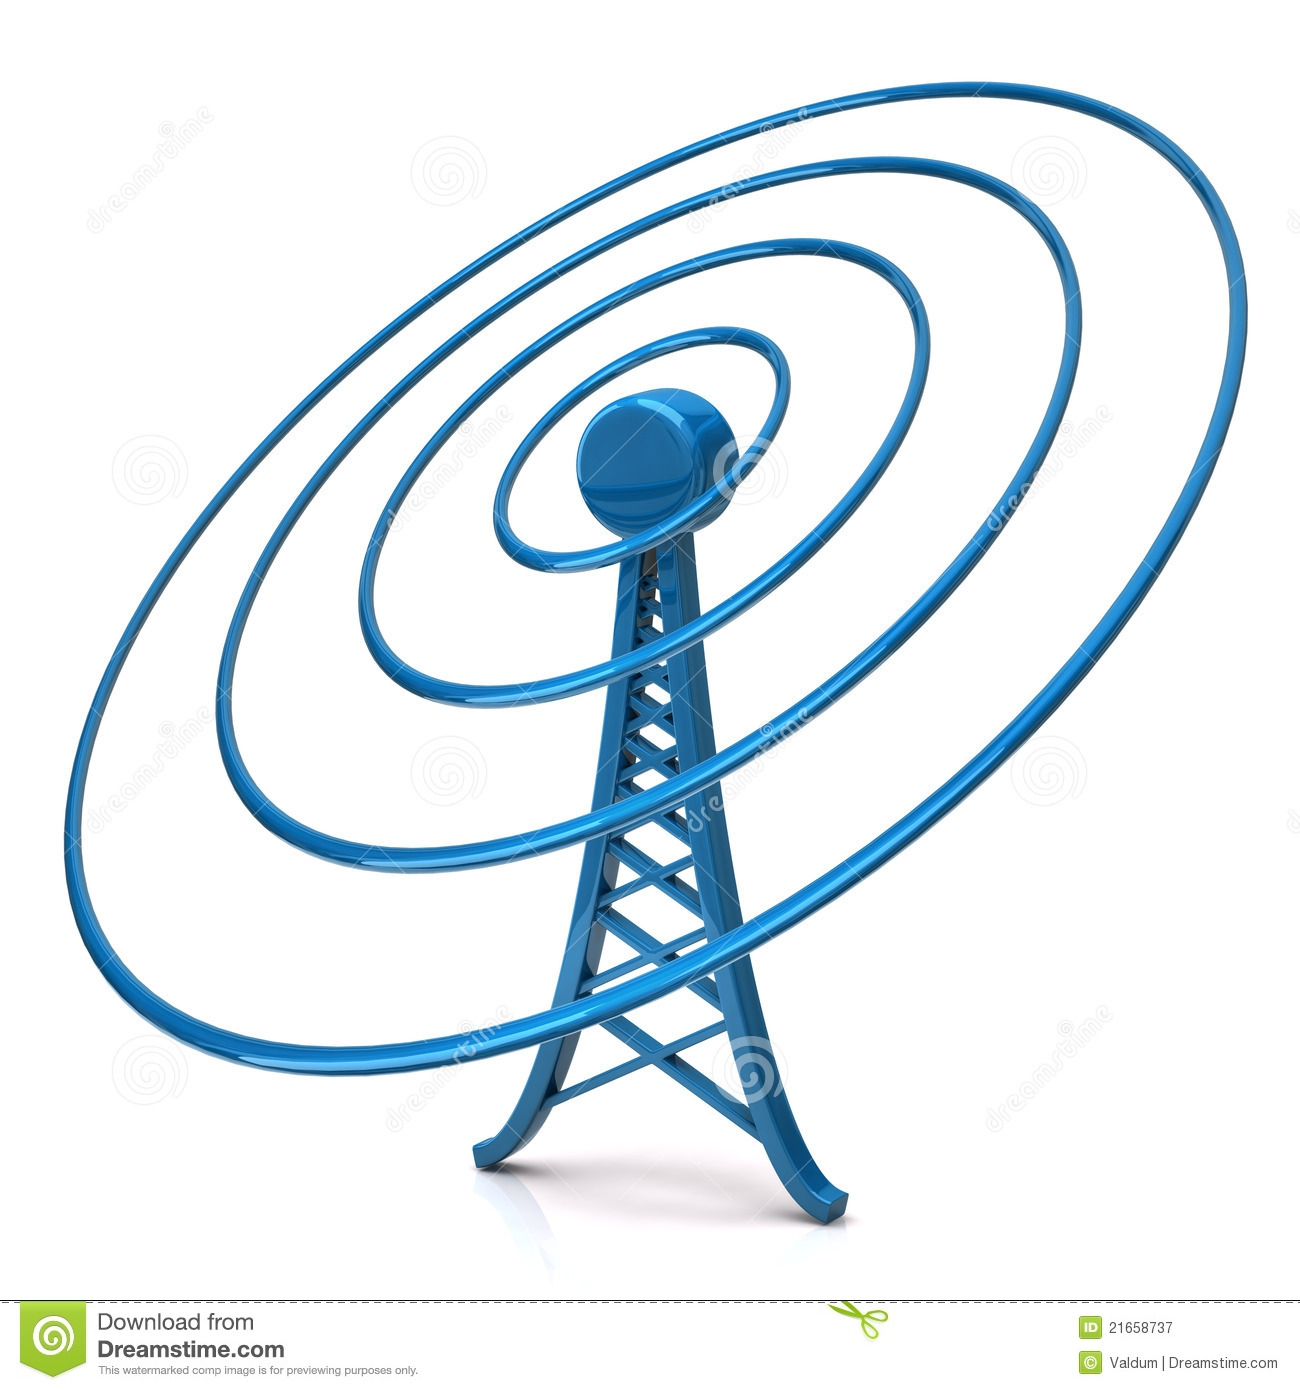
\includegraphics[height = 3cm]{tower.jpg}};
\filldraw[draw=white,fill=white] (4.5,11.25) rectangle (6.5,11.6);

\draw node at (6,11.2) {\textbf{SN(5G)}};

\draw [black, line width = 4pt] (6,11) -- (6,7.75);



\node[inner sep=0pt] (wsn) at (0,11.9)
    {
\includegraphics[height = 3cm]{smartphone.png}};
\draw node at (0,11.2) {\textbf{UE(5G)}};

\draw node at (1.6,13) {HN's public key: $\mathit{pk}$};


\draw [black, line width = 4pt] (0,11) -- (0,7.75);


\draw [black, line width = 4pt, ->] (6.0,10) -- (0,10);
\draw node at (3.0,10.4) {Reveal \textbf{IMSI}};


\draw [black, line width = 4pt, <-] (6,9) -- (0,9);
\draw node at (3,9.4) {$\text{MCC},\text{MNC},E_{\mathit{pk}}(\text{MSIN})$};

\draw [black, line width = 4pt, ->] (6,9) -- (12,9);
\draw node at (9,9.4) { $E_{\mathit{pk}}(\text{MSIN})$};

\draw [black, line width = 4pt, <-] (6,8) -- (12,8);
\draw node at (9,8.4) {MSIN};


\end{tikzpicture}


\end{center}



\section{Downgrade Attack}
\begin{Large} 5G phones will be interworking with LTE networks. So, an LTE based active IMSI catcher can still mount an attack.\end{Large}
\begin{center}
    \begin{tikzpicture}[scale=2.75]


\node[inner sep=0pt] (wsn) at (12,12)
    {
\includegraphics[height = 3cm]{home_network.jpg}};
\draw node at (12,11.2) {\textbf{HN (5G)}};

\draw [black, line width = 4pt] (12,11) -- (12,6.8);

\node[inner sep=0pt] (wsn) at (6,12)
    {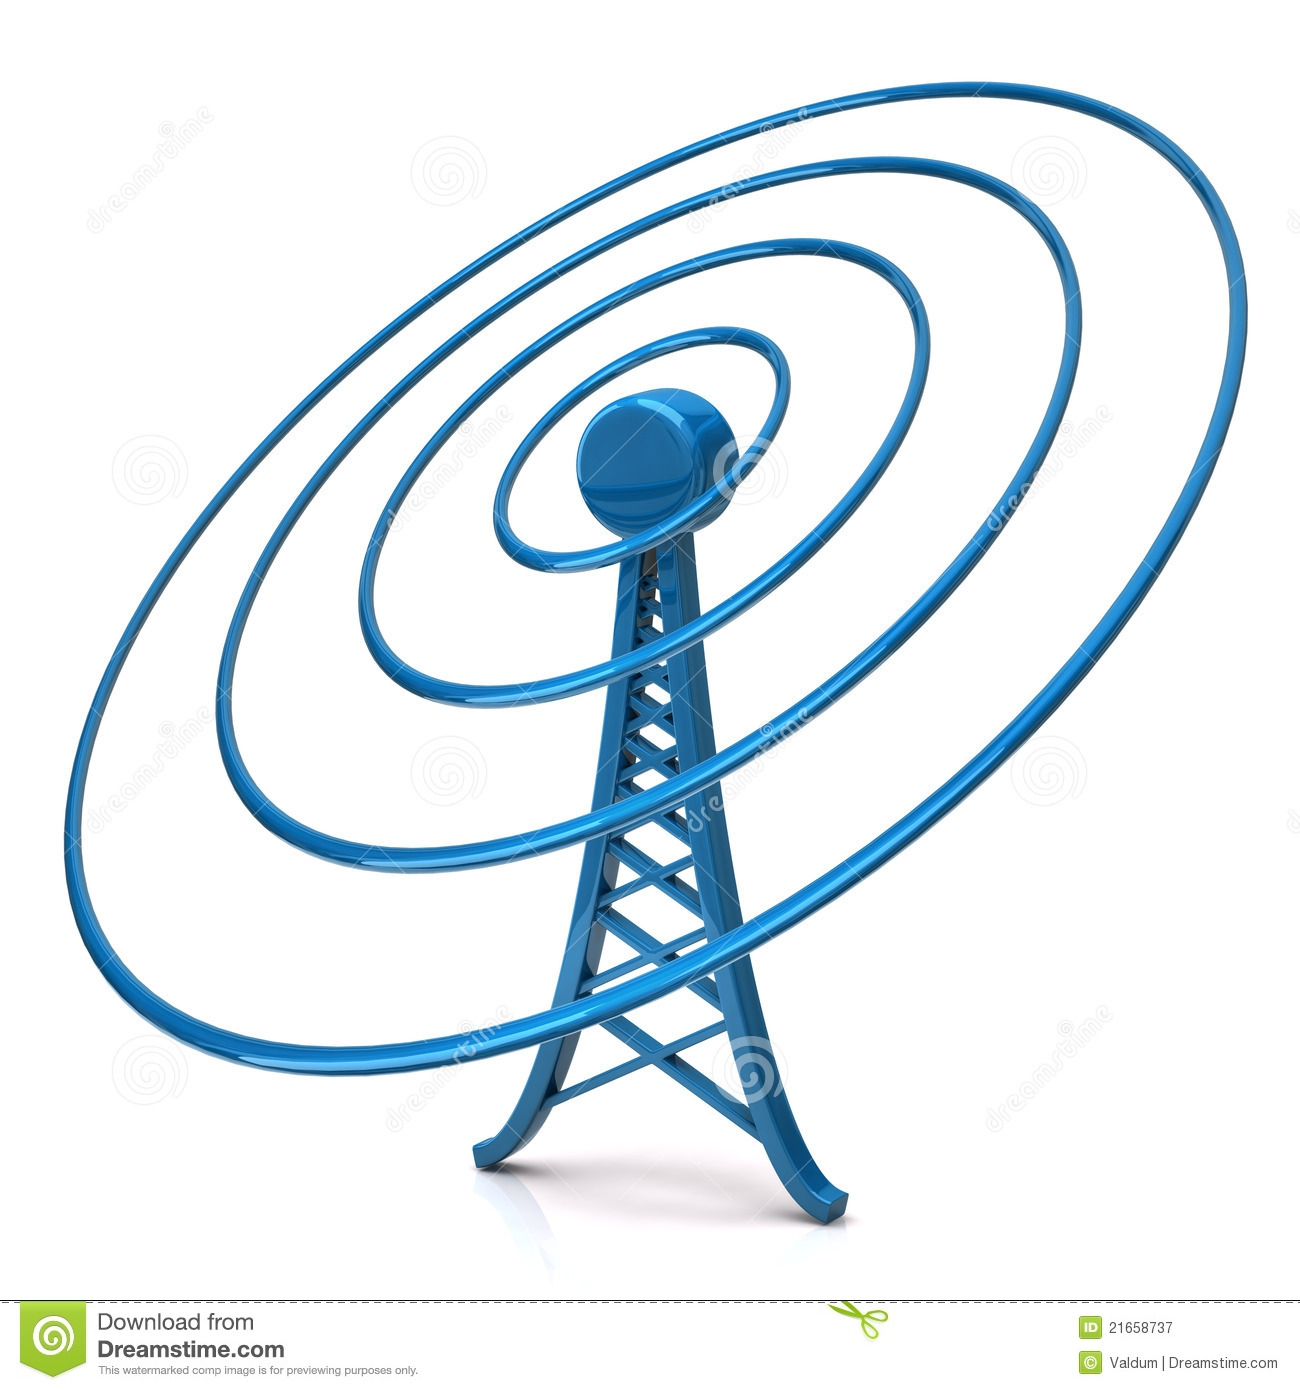
\includegraphics[height = 3cm]{tower.jpg}};
\filldraw[draw=white,fill=white] (4.5,11.25) rectangle (6.5,11.6);

\draw node at (6,11.2) {\textbf{SN(LTE/5G)}};

\draw [black, line width = 4pt] (6,11) -- (6,6.8);

\node[inner sep=0pt] (wsn) at (0,11.9)
    {
\includegraphics[height = 3cm]{smartphone.png}};
\draw node at (0,11.2) {\textbf{UE}};

\draw [black, line width = 4pt] (0,11) -- (0,6.8);


\draw [black, line width = 3pt, <->] (6.0,10) -- (0,10);
\draw node at (3.0,10.2) {\small Established connection};


\draw [black, line width = 4pt, ->] (3,9) -- (0,9);
\draw node at (1.5,9.5) {\small Stronger Signal};
\draw node at (1.5,9.2) {\small Reveal \textbf{IMSI}};

\draw [black, line width = 3pt, <->] (6.0,8) -- (0,8);
\draw node at (1.5,8) {\Huge \textcolor{red}{$\times$}};

\draw [black, line width = 4pt, <-] (3,7) -- (0,7);
\draw node at (1.5,7.2) {\small \textbf{IMSI}};


\node[inner sep=0pt] (wsn) at (3,12)
    {
\includegraphics[height = 3cm]{listening_tower.png}};
\draw [red, line width = 2pt,dotted,] (3,10.7) -- (3,6.8);
\draw node at (3,11.2) {\small \textbf{\textcolor{red}{Fake SN (LTE)}}};
\draw node at (3,10.9) {\small \textbf{\textcolor{red}{Active IMSI Catcher}}};

%\filldraw[-, dotted, fill opacity=0.2, cyan,line width = 3pt] (3,12.3) arc (90:450:2.5);


\end{tikzpicture}


\end{center}


\section{Defeating Downgrade Attack}
\begin{large}
 A hybrid solution using public-key encryption and pseudonyms. Significant amount of study have been performed on pseudonym based solutions to defeat IMSI catchers \cite{Norrman_Naslund_Dubrova_2016,Ginzboorg_Niemi_2016,CCS15,SSR15}. We propose a mixing of pseudonym and public-key encryption to defeat the downgrade attack.
\end{large}


\begin{center}
    \begin{tikzpicture}[scale=3]

\node[inner sep=0pt] (wsn) at (12.2,12)
    {
\includegraphics[height = 7cm]{home_network.jpg}};
\draw node at (12,10) {\textbf{Home Network (5G)}};

\draw node at (12,14.1) {\small Public Key: $\mathit{HN}_e$};
\draw node at (12.05,13.7) {\small Private Key: $\mathit{HN}_d$};

\node[inner sep=0pt] (wsn) at (8,12)
    {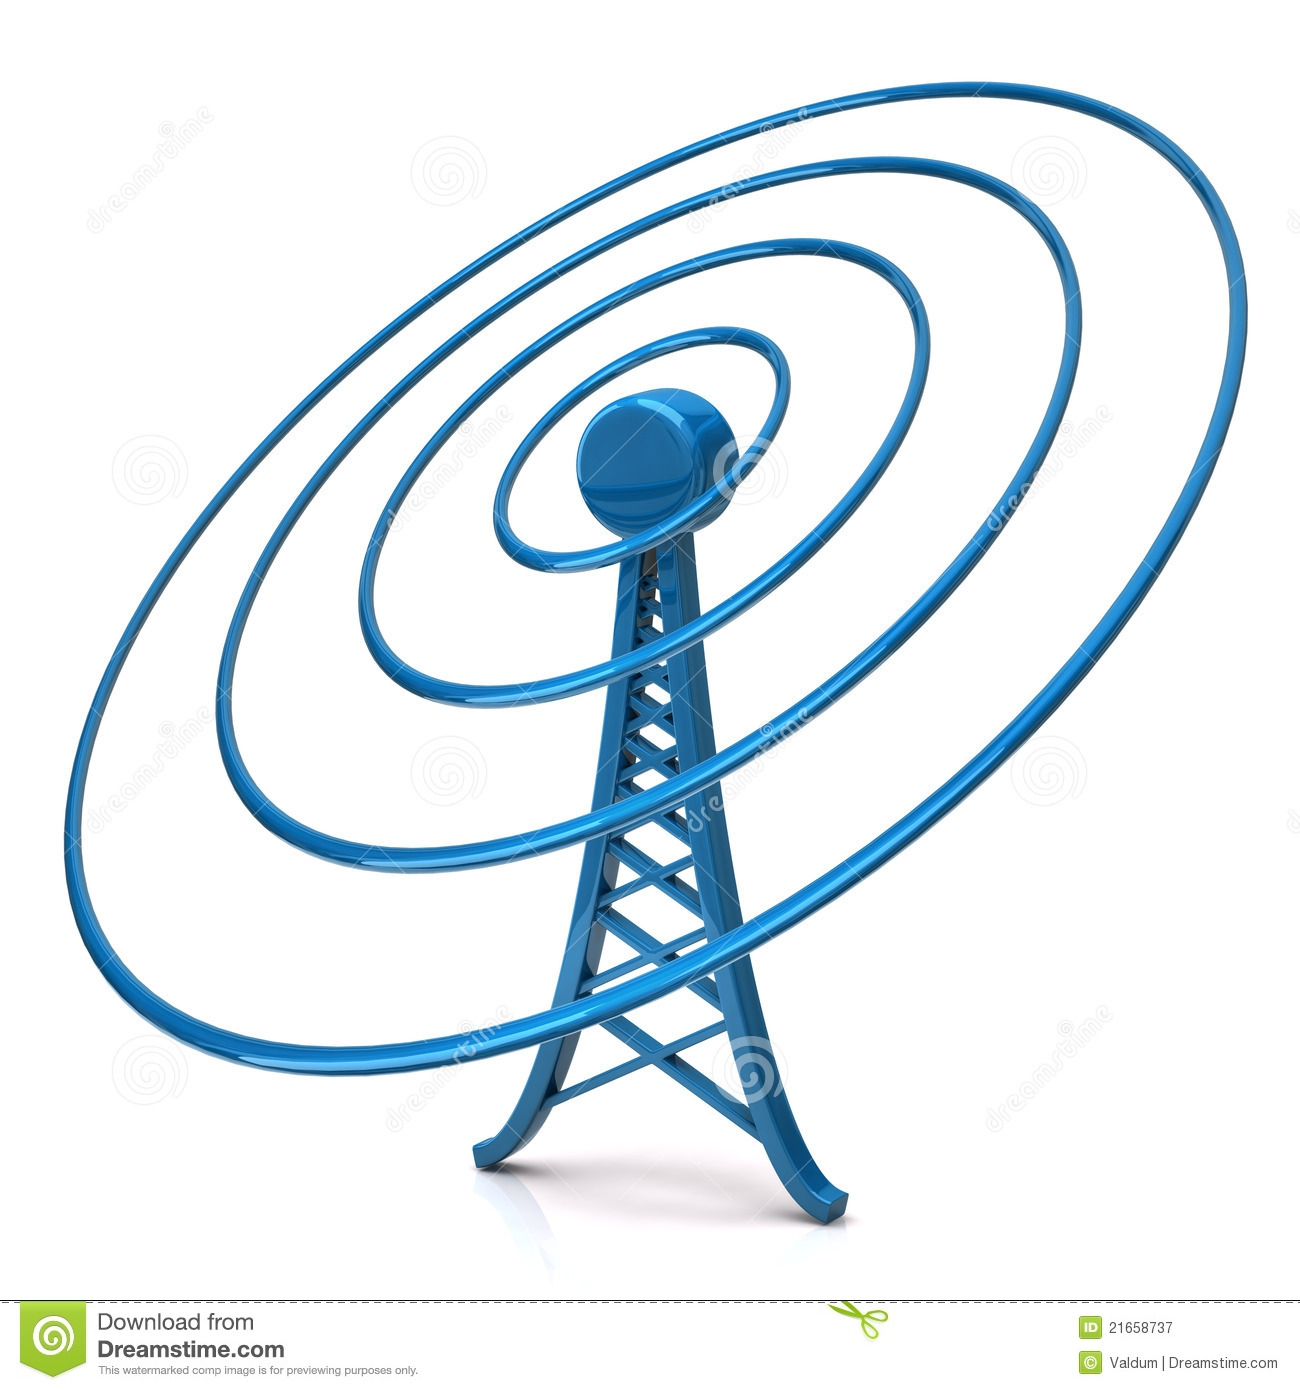
\includegraphics[height = 9cm]{tower.jpg}};

\draw node at (8,10) {\textbf{Serving Network (5G)}};

\filldraw[draw=white,fill=white] (6,10.25) rectangle (10,10.6);


\node[inner sep=0pt] (wsn) at (1,12)
    {
\includegraphics[height = 5cm]{smartphone.png}};


\draw [black, line width = 4pt, ->] (6.5,13) -- (1.8,13);
\draw node at (4.15,13.5) {\small Reveal \textbf{IMSI}};
\draw [black, line width = 4pt, <-] (6.5,12) -- (1.8,12);
\draw node at (4.15,12.3) {\small MCC||MNC||$E(\text{MSIN},\mathit{HN}_e)$};


\draw [black, line width = 4pt, ->] (9.2,12) -- (10.6,12);
\draw node at (9.9,12.3) {\small $E(\text{MSIN},\mathit{HN}_e)$};


\draw [black, line width = 4pt, <-] (9.2,11) -- (10.6,11);
\draw node at (9.9,11.3) {\small MSIN};


\end{tikzpicture}


\end{center}



%\normalsize

\bibliographystyle{plain}
\bibliography{ref}

\end{multicols}

\vfill % some more marginal in the end

\begin{minipage}[t]{0.9\linewidth} % footer
\footnotesize
\color{gray}{\textsf{\textbf{The {\LaTeX} template by Jussi Tiira used in this poster is licensed under a Creative Commons Attribution 4.0 International License.}}}
\end{minipage}


\end{document}
